\documentclass[../../main.tex]{subfiles}


\begin{document}
\subsection*{(a)}
Similarly to 1d), we created a new column chart. Here, we used the following Dimension:
\begin{verbatim}
CASE WHEN MATCH_PROCESS_REGEX("event_table_csv"."ACTIVITY", 'Closed'$) = 1
THEN CALC_THROUGHPUT(
	CASE_START TO CASE_END,
	REMAP_TIMESTAMPS("event_table_csv"."TIMESTAMP",HOURS)
)
ELSE CALC_THROUGHPUT(
	CASE_START TO LAST_OCCURRENCE['Resolve ticket'],
	REMAP_TIMESTAMPS("event_table_csv"."TIMESTAMP",HOURS)
)
END
\end{verbatim}
Using the Case Count as a Dimension, we got the following chart. Note that this is just a tiny section of the entire chart. There are cases with throughput times up to 1440h:\\
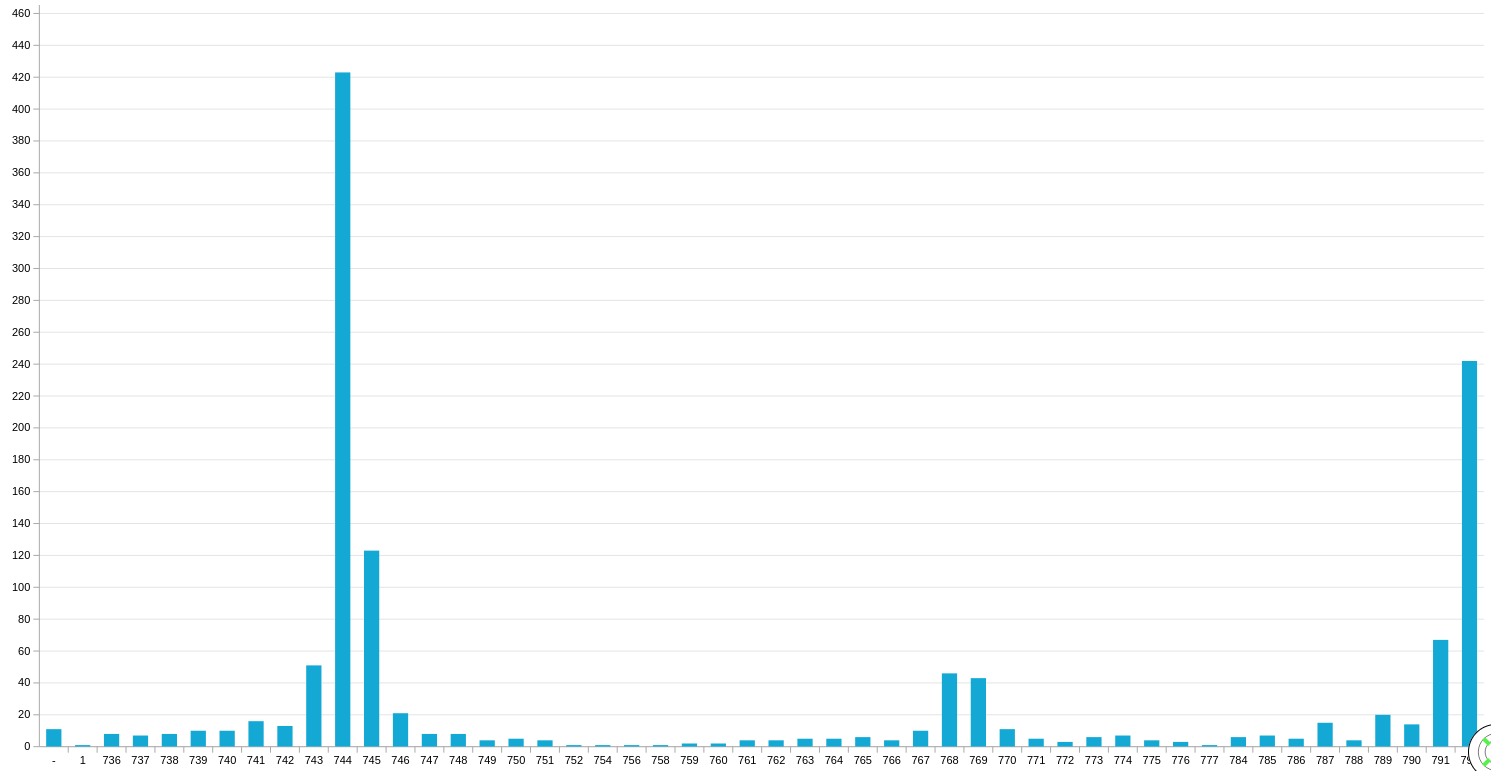
\includegraphics[width=\columnwidth]{img/Celonis_a_real_througput_times.png}


\subsection*{(b)}
We applied the \verb|Quantile| function on the real throughput times (see above) for 0.3 and 0.7, respectively.
For the 0.3-quantile we got 795h, for the 0.7-quantile 1079h.


\subsection*{(c)}
Approach equivalent to Question 4a). We used the following PQL queries:
\begin{verbatim}
	"case_table_csv"."CASE ID"
\end{verbatim}
\begin{verbatim}
	"case_table_csv"."TICKET TYPE"
\end{verbatim}
\begin{verbatim}
	"event_table_csv"."PRIORITY"
\end{verbatim}
\begin{verbatim}
CASE

WHEN (CASE WHEN MATCH_PROCESS_REGEX("event_table_csv"."ACTIVITY", 'Closed'$) = 1
THEN CALC_THROUGHPUT(
CASE_START TO CASE_END,
REMAP_TIMESTAMPS("event_table_csv"."TIMESTAMP",HOURS)
)
ELSE CALC_THROUGHPUT(
CASE_START TO LAST_OCCURRENCE['Resolve ticket'],
REMAP_TIMESTAMPS("event_table_csv"."TIMESTAMP",HOURS)
)
END) < 795 THEN 'Short'

WHEN (CASE WHEN MATCH_PROCESS_REGEX("event_table_csv"."ACTIVITY", 'Closed'$) = 1
THEN CALC_THROUGHPUT(
CASE_START TO CASE_END,
REMAP_TIMESTAMPS("event_table_csv"."TIMESTAMP",HOURS)
)
ELSE CALC_THROUGHPUT(
CASE_START TO LAST_OCCURRENCE['Resolve ticket'],
REMAP_TIMESTAMPS("event_table_csv"."TIMESTAMP",HOURS)
)
END) < 1079 THEN 'Medium'

ELSE 'Long'

END
\end{verbatim}
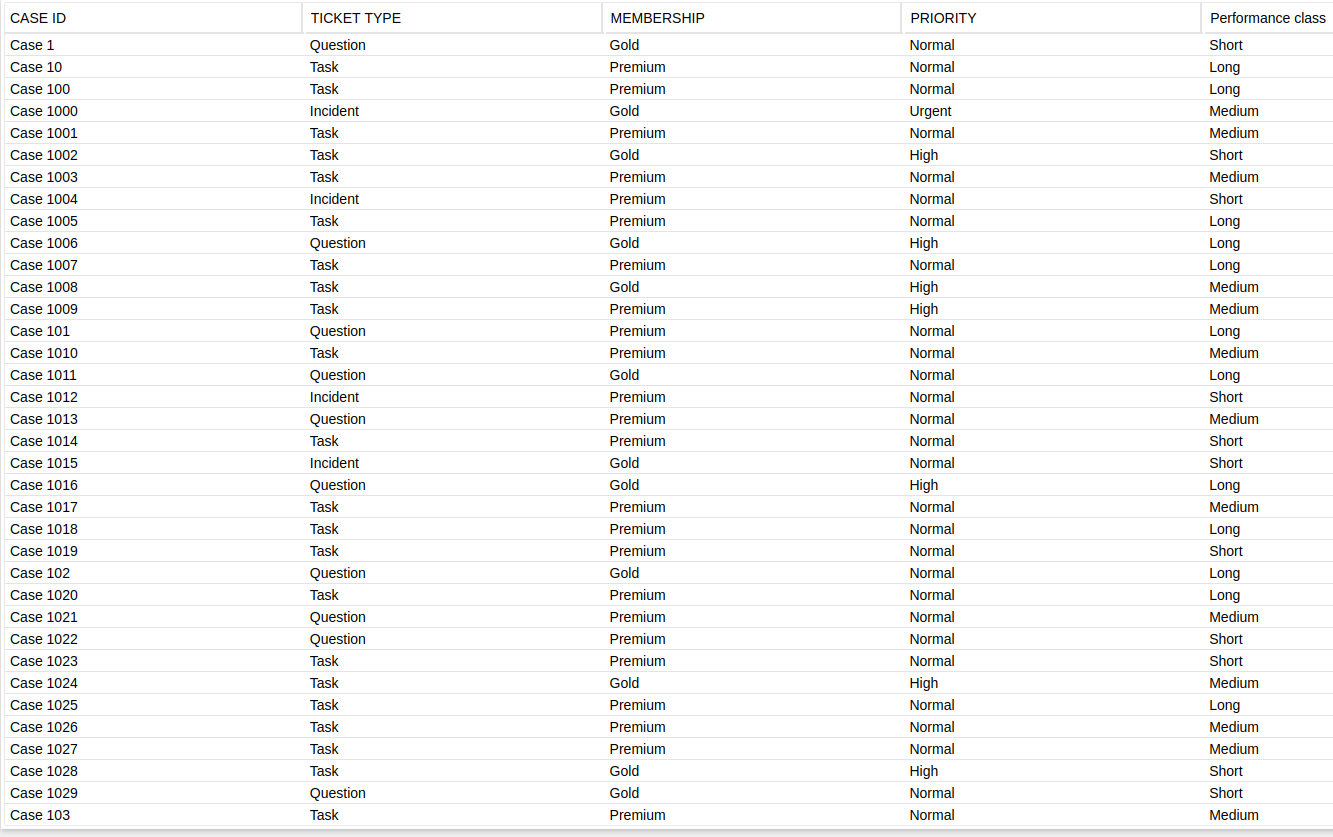
\includegraphics[width=\columnwidth]{img/Celonis_c_Olap.png}


\subsection*{(d)}
First, we export the OLAP Table and import it into RapidMiner as described in Instruction 2. Even after setting the parameters of the Decision Tree algorithm to extreme values (minimal gain at 1.0E-6), we could not find any clear variable that predicts the outcome of the performance class in any way. Thus, we conclude that the performance class (and thus the real throughput time) has no strong correlation with neither Priority nor Ticket Type. The only thing noticeable was, that close to half the Tasks stemming from Premium Memberships were Medium rated in real throughput time.


\end{document}